本次研究的数据集为~\verb|rumor.csv|,其中包含了366条谣言数据。鉴于数据背景、来源、变量含义以及预期目标已经在作业中给出,此处不再赘述。
在数据处理、分析前,我们将数据存储在~\verb|pandas.DataFrame|~类中,以便于后续的数据处理与可视化分析。

\subsection{数据预处理步骤}

在此节中,我们将对数据集进行预处理,为接下来的数据可视化分析打下基础。
首先,选取数据集的前5条谣言数据,观察数据集的部分内容及描述性统计,确定预处理数据的步骤。
数据集前5条谣言数据如表~\ref{tab:datasetContent}~所示。
数据集各变量在~\verb|DataFrame|~中的类型及部分描述性统计如表~\ref{tab:datasetVariable}~所示。

\begin{table}[!ht] \centering
    \begin{tabularx}{\linewidth}{X c c c c c c c}
        \toprule
        date & source & content & province & user\_0 & \dots & user\_17 & like \\
        \midrule
        2022-02-18 & 北京日报客户端 & 有人从香港\dots & 广东 & 0 & \dots & 0 & 0 \\
        2022-02-18 & 大河报、羊城晚报 & 近日,社交\dots & 河南 & 0 & \dots & 0 & 41 \\
        2022-02-17 & 南方都市报、大众网 & 近日,网传\dots & 湖南 & 0 & \dots & 0 & 26 \\
        2022-02-17 & 江苏省互联网举报中心 & 近日,网传\dots & 江苏 & 0 & \dots & 0 & 31 \\
        2022-02-16 & 中国新闻网 & 在塞企业机\dots & \color{red}{NaN} & 0 & \dots & 0 & 0 \\
        \bottomrule
    \end{tabularx}
    \caption{数据集前5条谣言数据}
    \label{tab:datasetContent}
\end{table}

\begin{table}[!ht] \centering
    \begin{tabularx}{\linewidth}{X c c c c c c c c}
        \toprule
        变量名 & date & source & content & province & user\_0 & \dots & user\_17 & like \\
        \midrule
        类型 & object & object & object & object & int64 & \dots & int64 & int64 \\
        非空值 & 366 & 360 & 366 & 277 & 366 & \dots & 366 & 366 \\
        均值 & - & - & - & - & 0.19 & \dots & 0.02 & 72.59 \\
        最小值 & - & - & - & - & 0 & \dots & 0 & 0 \\
        中位数 & - & - & - & - & 0 & \dots & 0 & 34 \\
        最大值 & - & - & - & - & 1 & \dots & 1 & 2495 \\
        \bottomrule
    \end{tabularx}
    \caption{数据集变量类型及部分描述性统计}
    \label{tab:datasetVariable}
\end{table}

分析表~\ref{tab:datasetContent}~和表~\ref{tab:datasetVariable}~内容,可以发现以下几个问题
\footnote{注意到数据集中user\_0到user\_17变量应该为Bool类型变量,但目前是int64类型的0-1变量,不妨碍分析。}:
% NOTE: 这一点不是很确定要不要写
\begin{enumerate}
    \item 数据集中source、province变量存在NaN值,需要对这些缺失值进行处理;
    \item 数据集中date变量应该为Datetime类型,但目前是object类型,需要进行类型转换才能进行与时间相关的分析;
    \item 数据集中like变量最小值、最大值差距很大,而中位数远小于均值,说明like变量的分布严重左偏。
\end{enumerate}

根据上述通过观察得到的问题,我们的预处理分为以下几个步骤\footnote{由于数据集中的每条谣言数据主要由谣言文本构成,因此不涉及离群值处理}:
\begin{enumerate}
    \item 数据缺失值处理。对于source、province变量的缺失值,
    由于谣言来源或涉及省份和谣言内容紧密相关,可以通过观察谣言内容结合搜索引擎,手动将这些缺失值填上;
    对于那些无法分辨出谣言来源或涉及省份时,填充数据或删除该条谣言数据都不合理,因此保留NaN值,
    在后续涉及source或province的分析过程中,忽略这些缺失值对应的谣言数据。
    \item 数据重复值处理。由于重复值的出现可能会影响分析结果,而数据集中谣言数量较小,可以通过观察法来判断数据集中是否存在重复值。
    % 如果存在重复值,则以谣言发布时间最早的为准。
    % NOTE: 如果有重复值,要写处理的方法
    \item 数据类型转换。将数据集中的date变量转换为Datetime类型。 % NOTE: user\_0到user\_17变量可能会改
    \item 变量数值变换。like变量与对like变量每个值取$\ln(x+1)$如图~\ref{fig:like_loglike_hist}~所示,
    从图中可以发现对like变量每个值取$\ln(x+1)$能更加接近正态,因此,可以对like变量每个值取$\ln(x+1)$并保存在新的变量log\_like中。
    \item 分词处理。将数据集中的content变量通过~\verb|jieba|~库进行分词处理。
    在分词时,利用自定义停用词表\footnote{停用词表位于文件\path{./data/stop_words}中}中的词作为停用词,不进行分词。
    分词后的结果(一个list)保存在新的变量content\_token中。 % NOTE: 可能source\_token没必要
\end{enumerate}

\begin{figure}[!ht]
    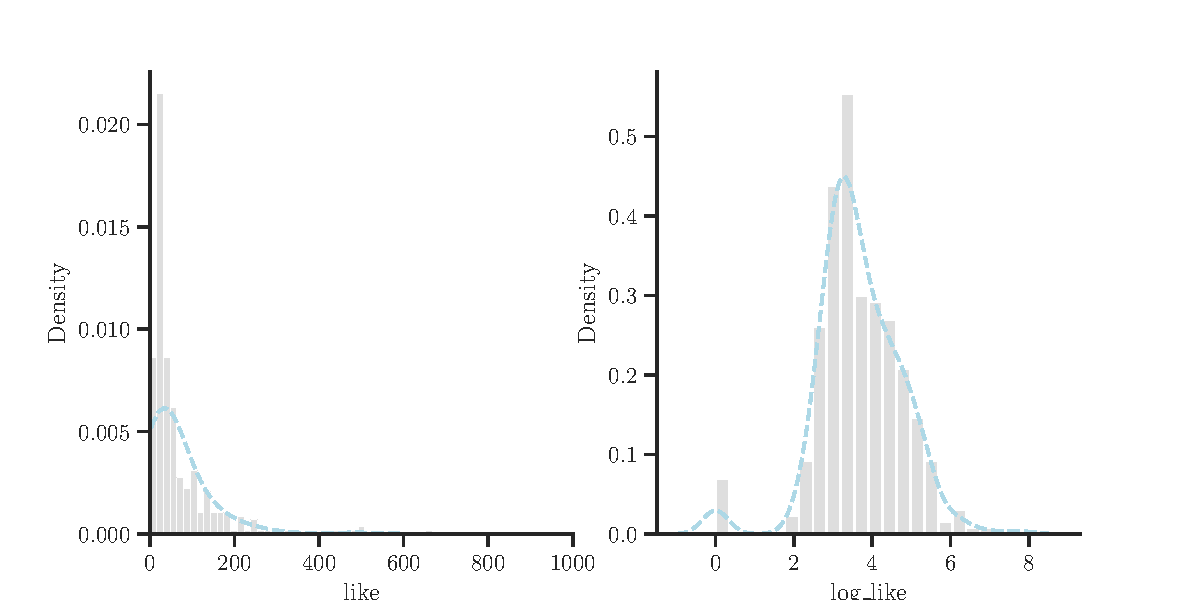
\includegraphics[width=\linewidth]{../figures/loglike_like_hist}
    \caption{like变量与log\_like变量的直方图}
    \label{fig:like_loglike_hist}
\end{figure}

\subsection{数据预处理结果}

根据上节提到的预处理步骤,我们对数据集进行了预处理。在数据预处理时,得到了以下结果:
\begin{enumerate}
    \item 由于谣言来源难以查找,填充了0个source变量缺失值;填充了32个province变量缺失值,这一变量的缺失值填充较为容易:
    例如第7条谣言数据的province变量为缺失值,谣言信息为“网传横州市马山镇太宁村有一阳性病例接触者?谣言!”,
    根据“横州市马山镇”的地理信息,可以判断该谣言涉及广西省,
    因此将原本的缺失值填充为“广西”。
    \item 数据集中不存在重复值。
    \item ~\verb|jieba|~库在处理地名时有分词问题,再以第7条谣言数据举例,分词结果为:[网传, 横, 州市, 马, 山镇, 太宁, 村有, 阳性, 病例, 接触, 谣言],
    但“横州市”、“太宁村”应该作为一个词。因此,我们需要对分词结果进行处理,纠正这一地名问题。
    但是具体地名在之后的分析过程不重要,对分析结果的影响不大,而处理地名问题十分复杂,收益远大于付出,因此我们不再对分词结果进行处理。
\end{enumerate}

预处理后的数据集部分内容如表~\ref{tab:datasetPreprocessedVariable}~所示。

\begin{table}[!ht] \centering
    \begin{tabularx}{\linewidth}{X c c c c c c c}
        \toprule
        变量名 & date & source & content & province & \dots & log\_like & content\_token \\
        \midrule
        类型 & datetime64[ns] & object & object & object & \dots & float64 & object \\
        非空值 & 366 & 360 & 366 & 309 & \dots & 366 & 366 \\
        均值 & 2021-12-20 & - & - & - & \dots & 3.67 & - \\
        最小值 & 2021-11-07 & - & - & - & \dots & 0 & -\\
        中位数 & 2021-12-20 & - & - & - & \dots & 3.55 & -\\
        最大值 & 2022-02-18 & - & - & - & \dots & 7.82 & -\\
        \bottomrule
    \end{tabularx}
    \caption{数据预处理后变量类型及部分描述性统计}
    \label{tab:datasetPreprocessedVariable}
\end{table}